\documentclass[12pt, twocolumn, oneside]{article}  	% use "amsart" instead of "article" for AMSLaTeX format
\usepackage[margin=.6in, top=1.2in]{geometry}                		% See geometry.pdf to learn the layout options. There are lots.                		% ... or a4paper or a5paper or ... 
\geometry{a4paper, landscape}                		% Activate for for rotated page geometry
%\usepackage[parfill]{parskip}    		% Activate to begin paragraphs with an empty line rather than an indent
\usepackage{graphicx}				% Use pdf, png, jpg, or eps§ with pdflatex; use eps in DVI mode
								% TeX will automatically convert eps ---> pdf in pdflatex		
\usepackage{amssymb}


\setlength{\columnsep}{10em}

\usepackage[none]{hyphenat}

\usepackage{fancyhdr}% http://ctan.org/pkg/fancyhdr
\pagestyle{fancy}
\lhead{\parbox{\columnwidth}{\textbf{\emph{\footnotesize Preludes to a Science of Insurrection}}}}
\rhead{\parbox{\columnwidth}{\textbf{\emph{\footnotesize}} \hfill\textbf{\footnotesize \thepage}}}
\cfoot{} % get rid of the page number 
\renewcommand{\headrulewidth}{0pt}
\renewcommand{\footrulewidth}{0pt}

%\usepackage{fontspec}
% \setmainfont{Palatino}

\title{Preludes}
\author{Justin Murphy}
\date{}							% Activate to display a given date or no date

\begin{document}
%\section{}
%\subsection{}

\setlength{\parindent}{0pt}


%\setlength{\parskip}{\baselineskip}

%\renewcommand\secheadstyle{\centering\Large\normalfont\noindent\textbf}

\newpage

\thispagestyle{empty}

%\section*{Page 12}

\vspace*{30em}


June 2015 \\
Southampton, UK

\newpage

\vspace*{1em}

\section*{\centering 28 Preludes to a Science of Insurrection}

\begin{center}

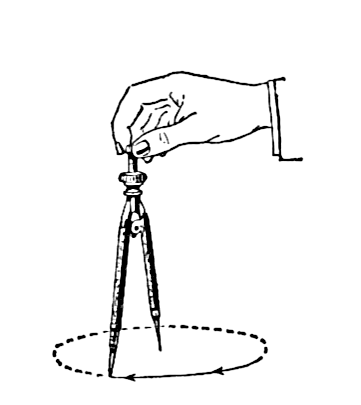
\includegraphics{compass.png}

\vspace*{3em}

\begin{large}
\textbf{Justin Murphy}
\end{large}

\begin{normalsize}
jmrphy.net/preludes \\
\end{normalsize}

\end{center}


\newpage

%\section*{Page 1}

The aphorism may have to become a genre of special importance to any sincerely radical intellectual, for the simple reason that anyone committed to writing down dangerous truths can only do so by snatching them quickly and irregularly from one's ever more fleeting and dwindling free time. Obviously the blog post as a genre testifies to this, but the mundane group psychology and attention economies of the web impose various conservative pressures on those who would try to think through blogging. When so much of our thought and feeling is pre-channeled into status quo institutions (thoughts and feelings which we subtly but irredeemably falsify as the price we pay to have them taken seriously by the relatively more powerful), one of the only ways to maintain an honest, living, dangerous intellectual project is to constantly overflow the cup of one's life---already filled to the brim by alienated work---and accumulate every little splash on any old rag at hand. Despite the unpolished, incomprehensible, inane, and even incorrect elements which will be inevitable, one's strung-together, splash-soaked rags will constitute a work of intellectual quality in crucial ways superior to most systematic works. While systematic works may be nicely filled cups, they are almost always funded by quotidian status quo hypocrisies which are required for their production but erased from the product; aphorisms are crystals formed on those splashes of honesty and truth squeezed out by such hypocrisies, preludes to something larger and more dangerous. In my life so far I have probably spent too much time making my silly little splashes and not enough tending the cup, but whether that has been my error, my crime, or my brilliance, only time will tell.

\newpage

%\section*{Page 10}
\setcounter{page}{10}
\renewcommand{\thepage}{\arabic{page}}

When all of one's ``free time'' is robbed, the entire social game of liberalism ends and becomes a race to the death. It implies certain parties to the social game of liberalism have been vanquished not only in the limited warfare of economic competition but altogether as human lives. Continuing to play such a game as if it is not already over brings a little bit of certain death every passing day. In contrast, each day one instead chooses to live is no longer a ``day off'' but a re-entry into the historical mortal combat from which liberal democracy was only a short-lived and illusory reprieve. This prospect is vertiginous until it is recalled one is already standing on the gallows. To risk death in a mad dash for freedom is certainly no more frightening; it only seems more frightening to those who do not think honestly about where they already stand. For it is only by choosing life that one can win a race to the death.

\vspace{3em}

I try to live so as to optimize the insurrectionary energy that would follow if I were unjustly killed, imprisoned, or disappeared. Another way to put this: I have been lucky enough to learn first hand that revolutionary politics is probably no more and no less than building true relationships and fighting to keep them. Incidentally, this is also one reason why the decline of organized religion has been a world-historical catastrophe, for whether we like it or not religion is the only basis humans have ever had, at least so far, for forging the kinds of relationships which make resistance to evil possible---that is, relationships which dare to exist on the level of life or death.

\newpage

%\section*{Page 10}

Multiple people will write with indignation, ``Why is nobody talking about X?''---pretending not to realize they are talking about X as soon as humanly possible after X happened. Why do they not just write something about it themselves and fill the gap they pretend to be concerned about? In most cases it is because they do not have anything new, interesting, or valuable to say, i.e. they are not talking about it for the same reason as those maligned for their silence, namely, nobody has anything worth saying because typically it is exceedingly hard and rare to find something worth saying. A thing is worth saying to the degree it feeds into some substantively active, living process of which it is a part. In an atomized and pacified society such as ours, writing and speaking are rarely if ever part of a truly living process. Therefore, it is very poorly appreciated the degree to which ``critical'' media personalities and even some of our most intelligent friends on social media already long ago quit the game of trying to say anything uniquely valuable. The typical ``hot take'' does not even try to convey new or unique information to its readers beyond the information they are already expected to have, i.e. such odd artifacts are sometimes literally, perfectly uninformative in the technical sense of the term. Well then, what are these people doing, from what land comes this fever in which one so loudly has nothing to say? Such heavy souls are selling affects for pocket change, whether symbolic or material---selling the very performance of their life---to then be pawned off by those others who possess even less ability to produce their own original affects, let alone new information. This may be all that is new in ``new media.''


\newpage

%\section*{Page 2}
\setcounter{page}{2}
\renewcommand{\thepage}{\arabic{page}}

To seek truth passionately does not imply one is uniquely capable of attaining it; so often such a passion is interpreted as arrogance. On the contrary, it indicates a uniquely energetic and honest form of modesty.

\vspace{3em}

I have no vision for the future of society but this does not make my political philosophy any less a world-historical, revolutionary rupture certain to change everything---for clearly it is!---it only means I am not a megalomaniac.

\vspace{3em}

Anyone who would wish to be an artist or intellectual is responsible for generating energy in others, an energy which is essentially ethical. As status quo institutions continue to strangle anyone childish enough to pursue such a task---as institutions have become exponentially more efficient since the information revolution---we observe nothing less than a society immunizing itself against the very possibility of becoming ethical. That such a remarkable process has also become so invisible, not even palpable by some of the most sensitive souls still around, only reflects how rapidly and completely several core human faculties have been destroyed in the course of about forty years.



\newpage

%\section*{Page 4}

State, party, faction, cadre,``safe space''---a lineage.

\vspace{3em}

There are still people on the radical left who do the selling newspapers thing. Just saying.

\vspace{3em}

Being who one truly is: always the most radical thing one can do, individually. At first this sounds trite, until one recalls that it invokes authenticity, a non-starter for many.

\vspace{3em}

Most of the benefits supposedly provided by status quo institutions fail to deliver their advertised satisfactions, but everyone goes on pretending to receive them, lest one be judged as incapable of happiness. The more success one has within the institutions, the more intense is this phenomenon. To have a comparatively decent perch in the world yet find almost all of its offerings unsatisfying appears as an absurd kind of ungratefulness. But this could not be more wrong: for people to traverse supposedly desirable stations and publicly out them for their emptiness is a first-class insurrectionary tactic. Such passings-through, which are also passings-over, concretely increase the truth and freedom of those touched while also leaving the enemy terrain even less habitable for all who will traverse it in the future.

\newpage

%\section*{Page 8}
\setcounter{page}{8}
\renewcommand{\thepage}{\arabic{page}}

In Barclay Shields I got out of my system in about one year what many other young adults are now inheriting as a norm overtaking the basic ethical substance of their lives, namely, that saying and doing things on the internet can feel good.

\vspace{3em}

I much prefer religious zealotry to vulgar atheism or so-called progressive religion, for only true zealotry can transcend the falsity of instrumental reason. In no way is this invalidated by  the promise of other-worldly rewards, which mean nothing and only serve as a bridge to allow the great mass of fallen mortals to fathom the otherwise incommensurable mode of life which is true religion. It always appears to others as if the believer must be driven by the instrumental purpose of obtaining some reward---but this is only because fallen mortals simply cannot access an experience of life beyond instrumental reason; that is what makes them fallen. The mortal thinks the believer is submitting to a primitive, traditional conception of reality in order to gain the benefits of a spiritual crutch in this world and fantastic rewards in the next, but the exact opposite is true: the faithful refuse to submit to the tyranny of empirical reality---the most insidious order of dishonest anesthesias and false prizes ever evolved---in favor of a \emph{true life now}, despite all indications against its possibility and with no guarantees of any rewards whatsoever.

\newpage

%\section*{Page 8}

There have been times I have fallen in love but then realized I was only inventing it precisely to avoid the disappointing fact that I was not falling in love. True love is no different, except one finally cares enough about the other to do this for eternity. In this, one finds a precious, secret joy which becomes a new reason to remain---perhaps, finally, a true one.

\vspace{3em}

Modernity, democracy, capitalism: elites pretend to relinquish power to individuals but really only relinquish direct control---in favor of institutional manipulations which only modulate aggregate distributions of behavior, in exchange for a net increase in power, which comes as a cut of the profits derived from the new, more efficient equilibrium.

\vspace{3em}

One can only have good character to the degree one is a character, in other words, an actor, a fake.

\vspace{3em}

Most people need money, not radical politics. Most ``radical'' politics need more people, not money.

\vspace{3em}

\newpage

%\section*{Page 4}
\setcounter{page}{4}
\renewcommand{\thepage}{\arabic{page}}

In the bourgeois professions it is hard to complain about work with a straight face, so the dissatisfactions pile up repressed behind smiles until the face grows weak and dull, for the face is no longer hiding a true self but rather revealing what one's self has truly become.

\vspace{3em}

Every generation eventually begins to suspect all is going to hell in a hand basket. The ignorant and the highly educated tend to agree in dismissing such pronouncements as unreliable, cyclical conservatism; because they have recurred like clockwork since time immemorial, such judgments are no longer seen as possibly indicating any real, new, objective degeneration of culture but only relative differences of perspective across generations. For this reason, neither the naive nor the ``critical" can take seriously all the implications of what now seems the most objectively likely possibility. Even after controlling for cyclical generational dynamics in perception, with every passing generation the world \emph{does} fall a little closer to hell, in a hand basket. Global warming indeed.

\vspace{3em}

Whenever I am with a group, I always ask myself: What degree of this is theater? If a lot, I stay. If very little, I stay. Otherwise, I run for the door.

\newpage

%\section*{Page 5}

I have made something, I have priced it at negative infinity, and I am smacking it out of your hand while saying ``if you break it, you buy it.''

\vspace{3em}

One must always keep the thread which runs from the beginning of one's life to the end. At any time, it can always be re-spun from whole cloth, but if one does not have---or cannot create---some thread running from the beginning to the end, this is the definition of being lost.

\vspace{3em}

Hatred will never be a liberating force without the generosity to love one's enemies, for it is only through generosity that one can desire to destroy the evil in someone \emph{for their own good}. One reason why theoretical critique as well as radical politics today cannot do very much is that people are far too happy to merely hate their enemies.

\vspace{3em}

Listening to someone whose ideas I cannot take seriously, I go into a daze which is kind and attentive but also akin to sleep; I become surrounded by a haze of fog, composed of love, contempt, self-righteousness, and nothingness---in what proportions I can never determine.

\vspace{3em}

Happiness derived from sunlight falsely inflates optimism; grey weather is depressing but grounding and for that reason more truthful.

\newpage

%\section*{Page 6}
\setcounter{page}{6}
\renewcommand{\thepage}{\arabic{page}}

Anyone who thinks social justice is more important than seeking the truth does not understand social justice and should be given what they are asking for: to be left alone.

\vspace{3em}

People do not get more conservative after they fall in love, they just gain something worth conserving. The old puzzle about how young revolutionaries so easily settle into politically tranquil family lives is not a puzzle: family is typically the most intensely communist organization possible in any society as atomized and pacified as ours. It is illusory to imagine that ``family values" are conservative and the revolutionary path requires infinite openness to unconstrained sexual exploration and flexibility of commitments, etc. The family is just one tactic among others and in many cases one family contains more revolutionary potential than most radical subcultures in the capitalist democracies.

\vspace{3em}

The more carefully one observes the police, the more one's hatred turns to pity and pity turns to contempt. Disinterested observation implies a privileged distance for sure; nonetheless, it is only when contempt then turns to laughter and forgetting that hatred of the police has completed itself. It is much better to spread the privilege necessary for this process to permeate the body politic than valorize as political culture a stillborn hatred little more than love turned bitter.



\end{document}  